\documentclass[letterpaper,11pt]{article}

\usepackage[spanish]{babel}
\usepackage[top=2cm,bottom=2cm,right=2cm,left=2cm]{geometry}
\usepackage{amssymb}
\usepackage{amsmath}
\usepackage{amsthm}
\usepackage{empheq}
\usepackage{mdframed}
\usepackage{booktabs}
\usepackage{lipsum}
\usepackage{graphicx}
\usepackage{color}
\usepackage{psfrag}
\usepackage{pgfplots}
\usepackage{bm}
\usepackage{multicol}
\usepackage{wrapfig}
\usepackage{float}
\usepackage{wrapfig}
\usepackage{multirow}
\usepackage{biblatex}
\usepackage{csquotes}
\usepackage{parskip}
\usepackage{cancel}
\usepackage{listing}
\usepackage{tikz}
\usepackage{verbatim}
\usepackage{subcaption}
\usepackage{enumitem}
\usepackage{xcolor}
\usepackage{xfrac}

\graphicspath{{fig/}}
\addbibresource{biblio.bib}
\usepgfplotslibrary{colorbrewer}
\pgfplotsset{width=8cm,compat=1.9}
\definecolor{negro}{RGB}{0,0,0}
\definecolor{azul}{RGB}{0,0,255}
\definecolor{verde}{RGB}{0,255,0}
\definecolor{cian}{RGB}{0,255,255}
\definecolor{rojo}{RGB}{255,0,0}
\definecolor{magenta}{RGB}{255,0,255}
\definecolor{amarillo}{RGB}{255,255,0}
\definecolor{blanco}{RGB}{255,255,255}

\definecolor{limegreen}{cmyk}{0.75,0,1,0}
\definecolor{orange}{cmyk}{0,0.8,0.95,0}
\definecolor{purple}{cmyk}{0.75,1,0,0}

\begin{document}

\onecolumn\begin{@twocolumntrue}
    \begin{minipage}{0.3\textwidth}{
\includegraphics[scale=0.24]{Escudo_UD.pdf}} % Cambiar escudo
    \end{minipage}
    \vspace{10pt}
    \begin{minipage}{0.677\textwidth}
        \begin{center}
            \vspace{12mm}
        
            \Large{\textbf{Tarea 3: osciladores y ecuaciones diferenciales}}
            \vspace{3mm}
            
            \large{\textbf{Juan Sebastian Manrique Moreno}}
            \vspace{2mm}
    
            \large{\textit{Ecuaciones diferenciales, Programa Académico de Física, Universidad Distrital Francisco José de Caldas}}
            \vspace{1mm}
            
            Octubre de 2022 % Formato (mes) de (año)
        \end{center}
\vspace{5pt}
\end{minipage}

\centerline{\rule{0.95\textwidth}{0.4pt}} % Línea negra
\end{@twocolumntrue}

\begin{multicols}{2}

\section*{Estimación computacional del potencial eléctrico de una línea circular de carga}

Se sabe que el potencial eléctrico, $V(\mathbf{r})$, de una línea circular de carga (ver Figura \ref{figenu:1}) de radio $R$ y densidad lineal de carga $\lambda$, viene dado por:
\begin{equation}
    V(\mathbf{r}) = \int\limits_{0}^{2\pi} \frac{k \lambda R d \theta}{\sqrt{\left(x-R\cos\theta\right)^{2}+\left(y-R\sin\theta\right)^{2}}} \label{ecuenu:1}
\end{equation}
A partir de la siguiente información realizar el siguiente experimento teórico:

\begin{figure}[H]
\begin{center}
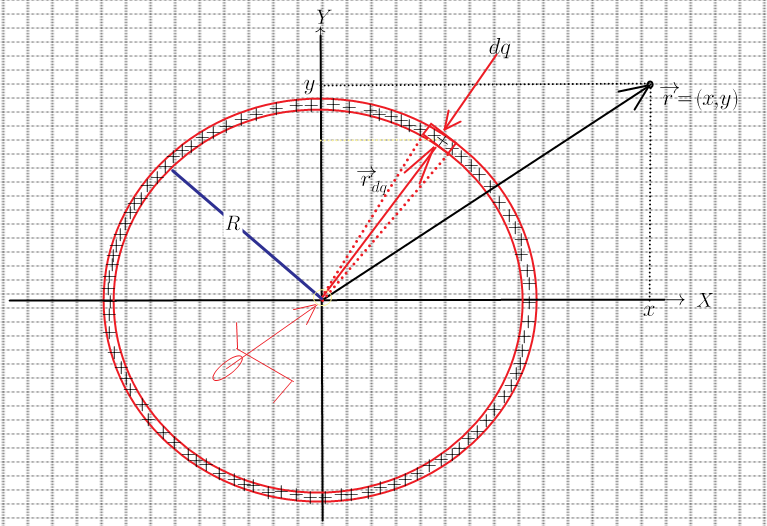
\includegraphics[width=0.485\textwidth]{img4.png}
\caption{Línea circular de carga}
\label{figenu:1}
\end{center}
\end{figure}

\begin{enumerate}[leftmargin=15pt]
    \item Suponer una línea circular de $R = 1.5~\mathrm{m}$, $\lambda = \frac{64 \times 10^{-9}}{3\pi} \frac{\mathrm{C}}{\mathrm{m}}$ y $k = 9 \times 10^{9}~\mathrm{N}\frac{\mathrm{m}^{2}}{\mathrm{C}^{2}}$.
    \item Realizar un bosquejo gráfico de la situación en una malla de $2 \times 2 \mathrm{m}$, ver Figura \ref{figenu:2}.
    \begin{figure}[H]
    \begin{center}
    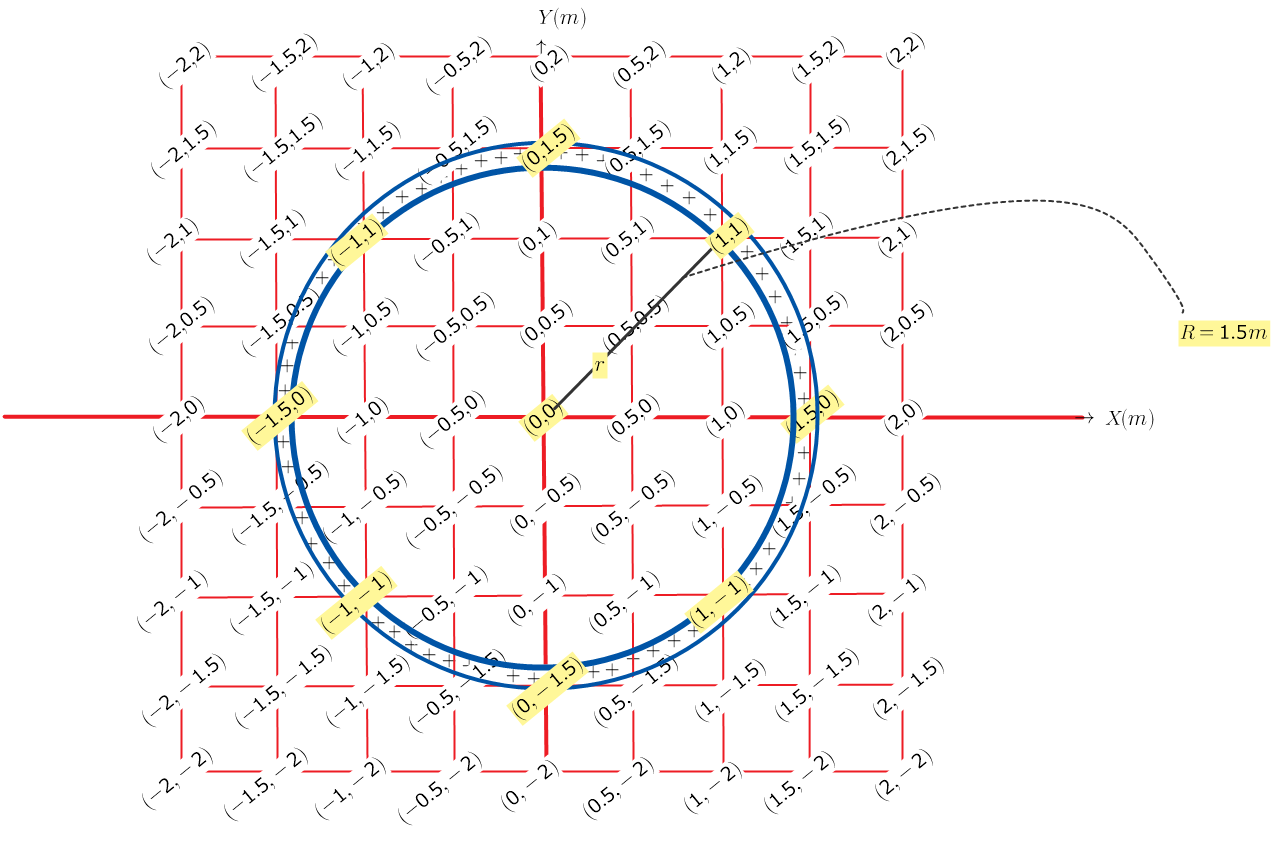
\includegraphics[width=0.485\textwidth]{img5.png}
    \caption{Bosquejo gráfico de la malla}
    \label{figenu:2}
    \end{center}
    \end{figure}
    \item Calcular el potencial que produce la línea circular de carga en los diferentes puntos de malla de $2 \times 2 \mathrm{m}$. Para tal fine evalúe la integral mostrada en (\ref{ecuenu:1}).
    \item Construir una tabla con los datos obtenidos.
    \item Represente gráficamente los datos del potencial eléctrico $V(x,y)$ la tabla, en función de las coordenadas $x$ y $y$. Para tal fin utilizar el software \textit{Surfer}.
    \item Con la misma tabla de datos del ítem anterior, representar las equipotenciales y las líneas de campo. Para tal fin utilizar el software \textit{Surfer}.
    \item Finalmente, realice una simulación con el \textit{Phet Interactive Simulation}, donde se muestre las equipotenciales y los vectores de campo. Ver Figura \ref{figenu:3}.
    \begin{figure}[H]
    \begin{center}
    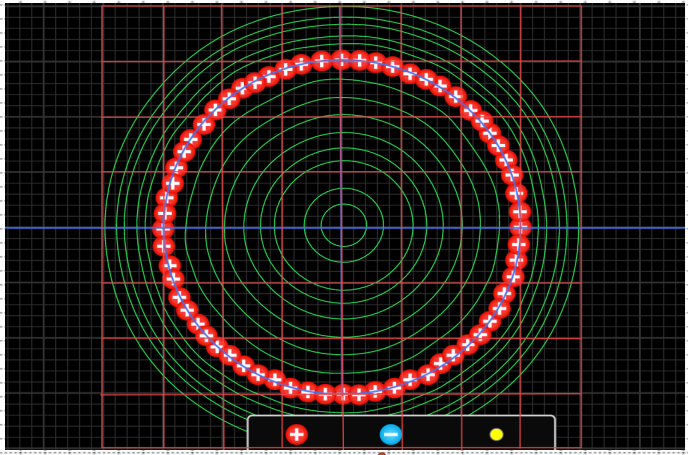
\includegraphics[width=0.485\textwidth]{img7.png}
    \caption{Sintaxis del laboratorio}
    \label{figenu:3}
    \end{center}
    \end{figure}
\end{enumerate}

\subsubsection*{Solución:}

La solución para este ejercicio no será ítem por ítem, sino que será de forma general.

Si supone una línea circular de la forma $R = 1.5~\mathrm{m}$, $\lambda = \frac{64 \times 10^{-9}}{3\pi} \frac{\mathrm{C}}{\mathrm{m}}$ y $k = 9 \times 10^{9}~\mathrm{N}\frac{\mathrm{m}^{2}}{\mathrm{C}^{2}}$, se plantean las mismas constantes en la integral expuesta en (\ref{ecuenu:1}), pero antes se va a desarrollar la integral en un álgebra por computador como lo es \textit{Wolfram Mathematica}.




\end{multicols}

\end{document}